% !TEX program = xelatex
\documentclass[twocolumn,10pt]{article}

% ==================== 中文支持 ====================
\usepackage{ctex}
\usepackage{fontspec}
\setmainfont{Times New Roman}
\setCJKmainfont{SimSun}[AutoFakeBold=2.0]

% ==================== 页面布局 ====================
\usepackage[top=2.54cm, bottom=2.54cm, left=2.0cm, right=2.0cm, columnsep=0.8cm]{geometry}

% ==================== 数学与物理 ====================
\usepackage{amsmath, amssymb, amsthm}
\usepackage{bm}
\usepackage{physics}

% ==================== 图表 ====================
\usepackage{graphicx}
\usepackage{float}
\usepackage{booktabs}
\usepackage{caption}
\usepackage{subcaption}

% ==================== 参考文献 ====================
\usepackage[sort&compress,numbers]{natbib}

% ==================== 超链接 ====================
\usepackage[colorlinks=true, linkcolor=blue, citecolor=blue, urlcolor=blue]{hyperref}

% ==================== 其他 ====================
\usepackage{enumitem}
\usepackage{abstract}
\usepackage{fancyhdr}

% ==================== 标题信息 ====================
\title{\vspace{-1.5cm}\textbf{N体轨道积分：太阳系简化模型与\\Leapfrog守恒性分析}\vspace{-0.3cm}}
\author{%
    \small
    徐浩祺%
    \quad
    肖羽 \\[3pt]
    \small 计算物理（含实验）课程 · 选题 A-2 · 2026 年春季学期
}
\date{}

% ==================== 摘要格式 ====================
\renewcommand{\abstractname}{\large\bfseries 摘\quad 要}
\renewcommand{\abstracttextfont}{\normalsize}

\begin{document}

\maketitle

% ==================== 摘要 ====================
\begin{abstract}
    本文使用显式Euler法和Leapfrog（速度Verlet）法两种数值积分格式，对太阳系简化N体模型进行了长期轨道积分模拟。
    通过太阳-地球两体系统的100年演化对比，定量分析了辛积分器与非辛积分器在能量守恒、角动量守恒方面的本质差异。
    收敛性测试验证了两种方法的实际精度阶数。
    作为拓展，本文在太阳-木星-小行星三体系统中观测到Kozai-Lidov机制，即小行星轨道偏心率和倾角的周期性耦合振荡，并验证了Kozai积分$\sqrt{1-e^2}\cos i$的准守恒性质。
    结果表明：Euler法在100年后能量漂移达$6.6\times 10^{-1}$，而Leapfrog法的相对能量误差始终维持在$10^{-14}$量级；两者的真实误差比超过$10^{13}$，充分证明了辛积分器在长期天体力学模拟中不可替代的核心地位。

    \textbf{关键词：}N体问题；辛积分器；Leapfrog算法；能量守恒；Kozai-Lidov机制；天体力学
\end{abstract}

% ==================== 1 引言 ====================
\section{引言}

N体问题是经典天体力学中最基本也最具挑战性的问题之一。自牛顿提出万有引力定律以来，两体问题已被完全解决——开普勒椭圆轨道给出了完美的解析描述。然而，当系统中存在三个或更多天体时，运动方程不再有封闭解析解，必须依赖数值方法求解\cite{murray1999solar, zingale2024astro}。

数值积分N体系统面临一个核心困难：长时间的轨道演化对数值格式的保结构性质极为敏感。一般的显式方法（如Euler法）虽实现简单，但不具备辛（symplectic）性质，每一步都会系统性地破坏相空间体积，导致能量单调漂移，轨道出现物理上不存在的螺旋扩张或收缩\cite{hairer2006geometric}。而辛积分器通过保持哈密顿系统的几何结构，使得能量在真实值附近有界振荡，无长期漂移，成为天体力学长期模拟的标准工具\cite{yoshida1990construction}。

本文选取太阳系简化模型作为研究对象，设计以下三组数值实验：(1) 太阳-地球两体系统，使用Euler法和Leapfrog法分别积分100年，对比轨道形态、能量守恒和角动量守恒；(2) 固定10年模拟时长下的收敛性测试，通过变化时间步长验证两种方法的实际精度阶数；(3) 太阳-木星-小行星三体系统，使用Leapfrog法积分500年，研究Kozai-Lidov效应。

本文的目的不仅是演示两种积分器的数值性能差异，更希望揭示其背后深刻的几何根源——辛结构保持是长期动力学模拟正确性的必要条件。

% ==================== 2 物理模型 ====================
\section{物理模型与控制方程}

\subsection{N体运动方程}

考虑$N$个质量为$m_i$的天体，其运动服从牛顿万有引力定律和牛顿第二定律。第$i$个天体的加速度为：

\begin{equation}
    \mathbf{a}_i = \frac{d^2\mathbf{r}_i}{dt^2}
    = \sum_{j \neq i}^{N} G\frac{m_j}{r_{ij}^3}\,\mathbf{r}_{ij},
    \label{eq:nbody}
\end{equation}

其中$\mathbf{r}_{ij} \equiv \mathbf{r}_j - \mathbf{r}_i$是天体$j$相对天体$i$的位置矢量，$r_{ij} = |\mathbf{r}_{ij}|$是二者之间的距离，$G$是万有引力常数。

为防止天体过分接近时引力趋于无穷导致的数值奇点，在分母中引入软化参数$\varepsilon$：

\begin{equation}
    \mathbf{a}_i = \sum_{j \neq i}^{N} \frac{G\,m_j\,\mathbf{r}_{ij}}
    {(r_{ij}^2 + \varepsilon^2)^{3/2}}.
    \label{eq:nbody_soft}
\end{equation}

本文取$\varepsilon = 10^{-4}$ AU，该值远小于天体间的最小距离，不影响物理结果，但有效防止了数值溢出。

\subsection{单位系统}

采用天体力学中常用的无量纲单位制：
\begin{equation}
    [L] = 1\ \text{AU},\quad
    [M] = 1\ M_\odot,\quad
    [T] = 1\ \text{yr}.
\end{equation}

在此单位制下，地球轨道的半长轴$a_\oplus = 1$ AU，轨道周期$P_\oplus = 1$ yr，万有引力常数简化为：

\begin{equation}
    G = 4\pi^2\ \text{AU}^3\,M_\odot^{-1}\,\text{yr}^{-2}.
\end{equation}

\subsection{守恒量}

保守力学系统的核心判据包括：

总机械能（动能$+$引力势能）：
\begin{equation}
    E = \sum_{i=1}^{N} \frac{1}{2}m_i v_i^2
    - \sum_{i<j} \frac{G\,m_i m_j}{r_{ij}}.
    \label{eq:energy}
\end{equation}

总角动量矢量：
\begin{equation}
    \mathbf{L} = \sum_{i=1}^{N} m_i\,(\mathbf{r}_i \times \mathbf{v}_i).
    \label{eq:angmom}
\end{equation}

对于保守系统，$E$和$\mathbf{L}$均应严格守恒。数值积分中两者的漂移量是衡量方法质量的核心指标。

\subsection{辛几何条件}

哈密顿系统的演化可看作相空间$(q,p)$上的正则变换。当且仅当数值映射保持相空间的辛2-形式$\omega = \sum_i dq_i \wedge dp_i$不变时，称之为辛积分器\cite{hairer2006geometric}。辛积分器的关键特征是：数值哈密顿量$\tilde{H}$（由积分器隐式定义）严格守恒，而原哈密顿量$H$在$\tilde{H}$附近有界振荡，因此能量无长期漂移。

非辛方法（如显式Euler）每步都会改变相空间体积元，相当于系统性地注入或抽取伪能量，导致能量单调演化\cite{springel2005simulating}。

% ==================== 3 数值方法 ====================
\section{数值方法}

\subsection{显式 Euler 法（一阶，非辛）}

Euler法是最简单的常微分方程数值解法。对于一阶系统$\dot{\mathbf{y}} = \mathbf{f}(\mathbf{y})$，其迭代格式为：

\begin{equation}
    \mathbf{y}_{n+1} = \mathbf{y}_n + \mathbf{f}(\mathbf{y}_n)\,\Delta t.
\end{equation}

应用于N体问题（位置-速度二阶系统）：

\begin{subequations}
\begin{align}
    \mathbf{v}_{n+1} &= \mathbf{v}_n + \mathbf{a}_n\,\Delta t, \label{eq:euler_v}\\
    \mathbf{r}_{n+1} &= \mathbf{r}_n + \mathbf{v}_n\,\Delta t. \label{eq:euler_r}
\end{align}
\end{subequations}

Euler法的局部截断误差为$\mathcal{O}(\Delta t^2)$，全局误差为$\mathcal{O}(\Delta t)$，故为一阶精度。其本质缺陷在于信息滞后：位置更新使用旧速度$\mathbf{v}_n$而非新速度$\mathbf{v}_{n+1}$，破坏了时间反演对称性，导致辛结构的丧失。

\subsection{Leapfrog / 速度 Verlet 法（二阶，辛）}

速度Verlet算法是Leapfrog格式的等价形式，通过对称化的半步交错实现辛性质：

\begin{subequations}
\begin{align}
    \mathbf{v}_{n+1/2} &= \mathbf{v}_n + \tfrac{1}{2}\mathbf{a}_n\,\Delta t, \label{eq:lf_halfv}\\
    \mathbf{r}_{n+1} &= \mathbf{r}_n + \mathbf{v}_{n+1/2}\,\Delta t, \label{eq:lf_pos}\\
    \mathbf{a}_{n+1} &= \mathbf{f}(\mathbf{r}_{n+1}), \label{eq:lf_acc}\\
    \mathbf{v}_{n+1} &= \mathbf{v}_{n+1/2} + \tfrac{1}{2}\mathbf{a}_{n+1}\,\Delta t. \label{eq:lf_fullv}
\end{align}
\end{subequations}

式(\ref{eq:lf_halfv})将速度推向半步中点；式(\ref{eq:lf_pos})用中点速度更新位置；式(\ref{eq:lf_acc})在新位置计算加速度；式(\ref{eq:lf_fullv})完成速度的同步更新。该格式具有时间反演对称性（即向前积分$k$步再反向积分$k$步能精确回到初态），这是辛性质的直接体现。局部截断误差为$\mathcal{O}(\Delta t^3)$，全局误差为$\mathcal{O}(\Delta t^2)$，达到二阶精度\cite{verlet1967computer}。

\subsection{软化参数选取}

式(\ref{eq:nbody_soft})中的软化参数$\varepsilon$模拟以下物理情境：(1) 真实天体有有限半径，不会坍缩为质点；(2) 在紧邻遭遇时，有限时间步长无法分辨快速变化的引力场。$\varepsilon$的选取需权衡：过大会扭曲远距离的引力场（有效势$-\!Gm/\sqrt{r^2+\varepsilon^2}$在$r \gg \varepsilon$时的误差为$\mathcal{O}(\varepsilon^2/r^2)$），过小则无法防止$r\to0$时的数值发散。

\subsection{轨道根数追踪}

为研究Kozai-Lidov机制，需从瞬时位置和速度中提取密切（osculating）开普勒轨道根数\cite{murray1999solar}：

\begin{align}
    \varepsilon_{\text{spec}} &= \frac{v^2}{2} - \frac{\mu}{r}, &
    a &= -\frac{\mu}{2\varepsilon_{\text{spec}}}, \label{eq:kepler_a}\\[4pt]
    \mathbf{e} &= \frac{\mathbf{v}\times\mathbf{h}}{\mu} - \frac{\mathbf{r}}{r}, &
    e &= |\mathbf{e}|, \label{eq:kepler_e}\\[4pt]
    \cos i &= \frac{h_z}{|\mathbf{h}|}, \label{eq:kepler_i}
\end{align}

其中$\mu = G(m_{\text{central}} + m_{\text{body}})$，$\mathbf{h} = \mathbf{r} \times \mathbf{v}$为比角动量。这些瞬时根数在扰动系统中会随时间缓慢变化，反映外界天体的引力扰动。

% ==================== 4 结果与分析 ====================
\section{模拟结果与分析}

\subsection{两体系统：轨道形态对比}

\begin{figure}[H]
    \centering
    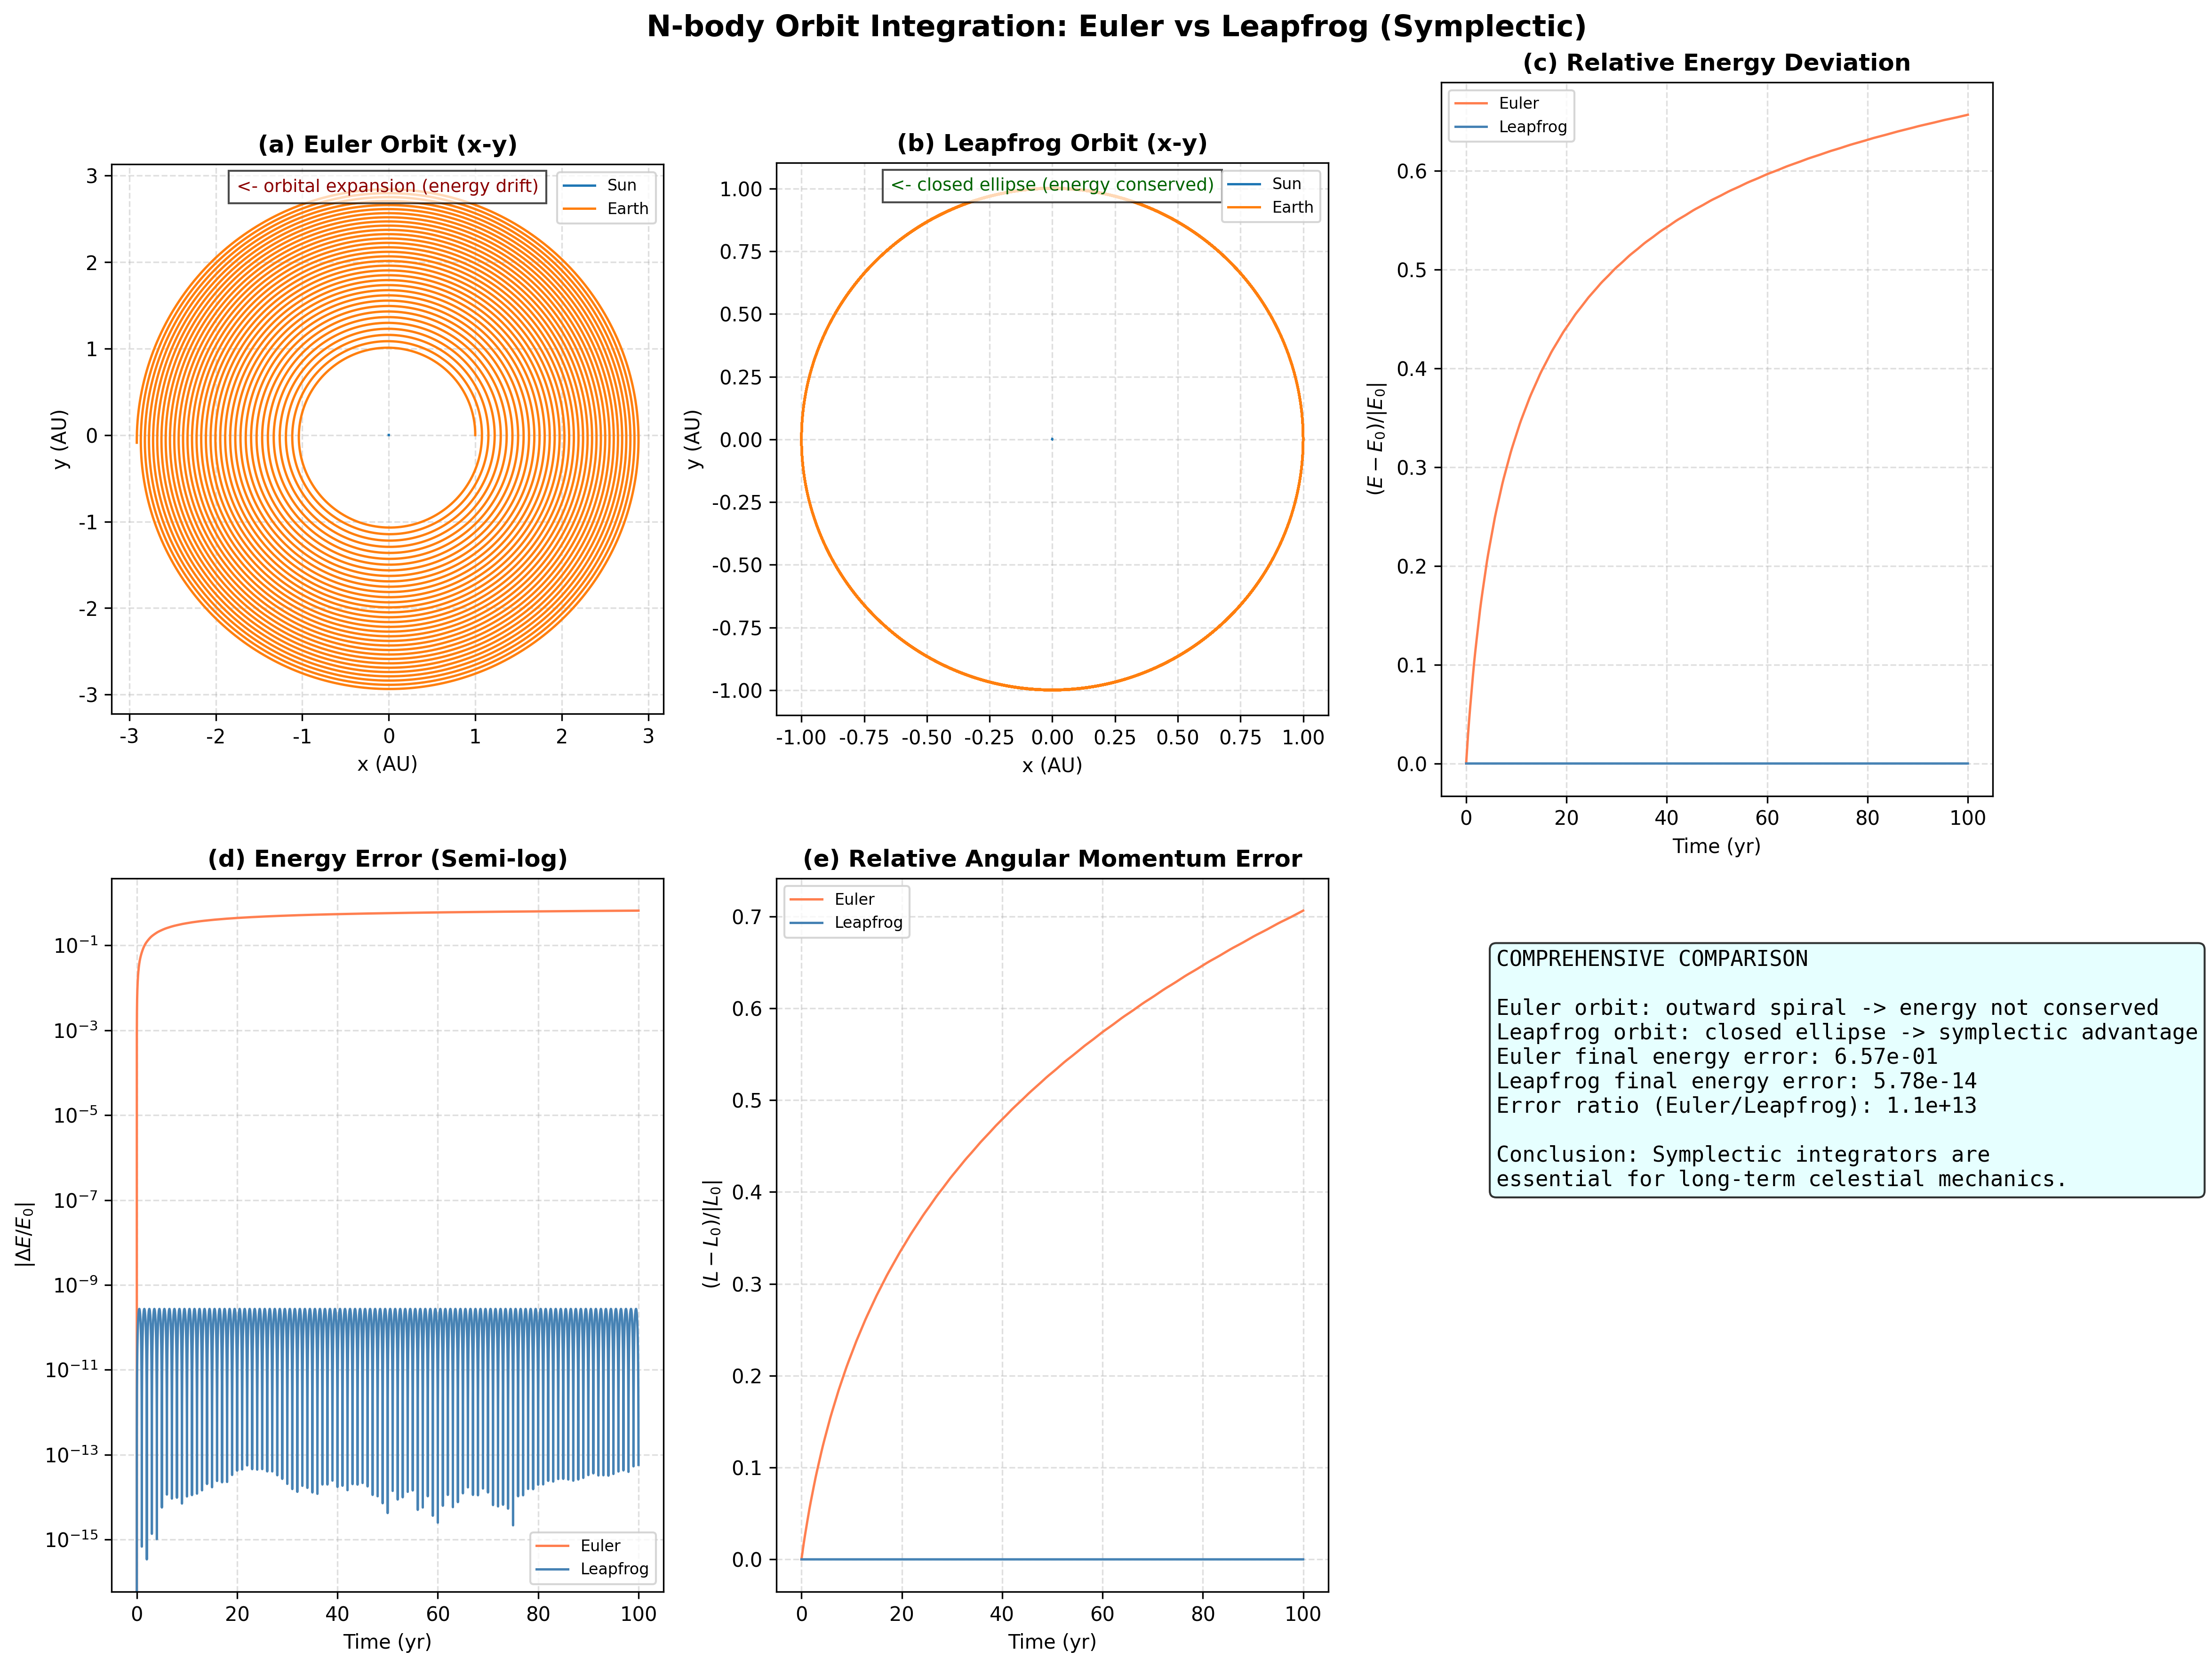
\includegraphics[width=\columnwidth]{assets/comprehensive_2body.png}
    \caption{两体系统综合对比面板。(a) Euler法轨道呈现明显的外螺旋扩张；(b) Leapfrog法保持闭合椭圆；(c)--(d) 相对能量偏差与半对数能量误差；(e) 角动量相对误差；(f) 数值对比总结。\\
    模拟参数：$\Delta t = 0.001$ yr，$T = 100$ yr，每轨道约1000步。}
    \label{fig:comprehensive}
\end{figure}

图\ref{fig:comprehensive}以六合一综合面板展示了太阳-地球两体系统100年模拟的核心结果。图(a)--(b)分别显示了Euler法和Leapfrog法下的x-y轨道投影。

Euler法的轨道（图a）呈明显的向外螺旋扩张——这并非真实的轨道演化，而是非辛积分引入的系统性能量伪影。每步积分中，位置更新式(\ref{eq:euler_r})使用的$\mathbf{v}_n$落后于加速度的瞬时变化，导致离心力被高估，天体获得额外的径向速度分量。这种人为的能量注入随时间累积，使得轨道半径不断增大。

Leapfrog法的轨道（图b）则保持完美的闭合椭圆——这正是Kepler第一定律所预言的太阳系行星运动。即使经过100年（100个轨道周期），轨道形状与初始条件几乎不可区分，直观地验证了辛积分器的长期稳定性。

\subsection{两体系统：能量守恒分析}

\begin{figure}[H]
    \centering
    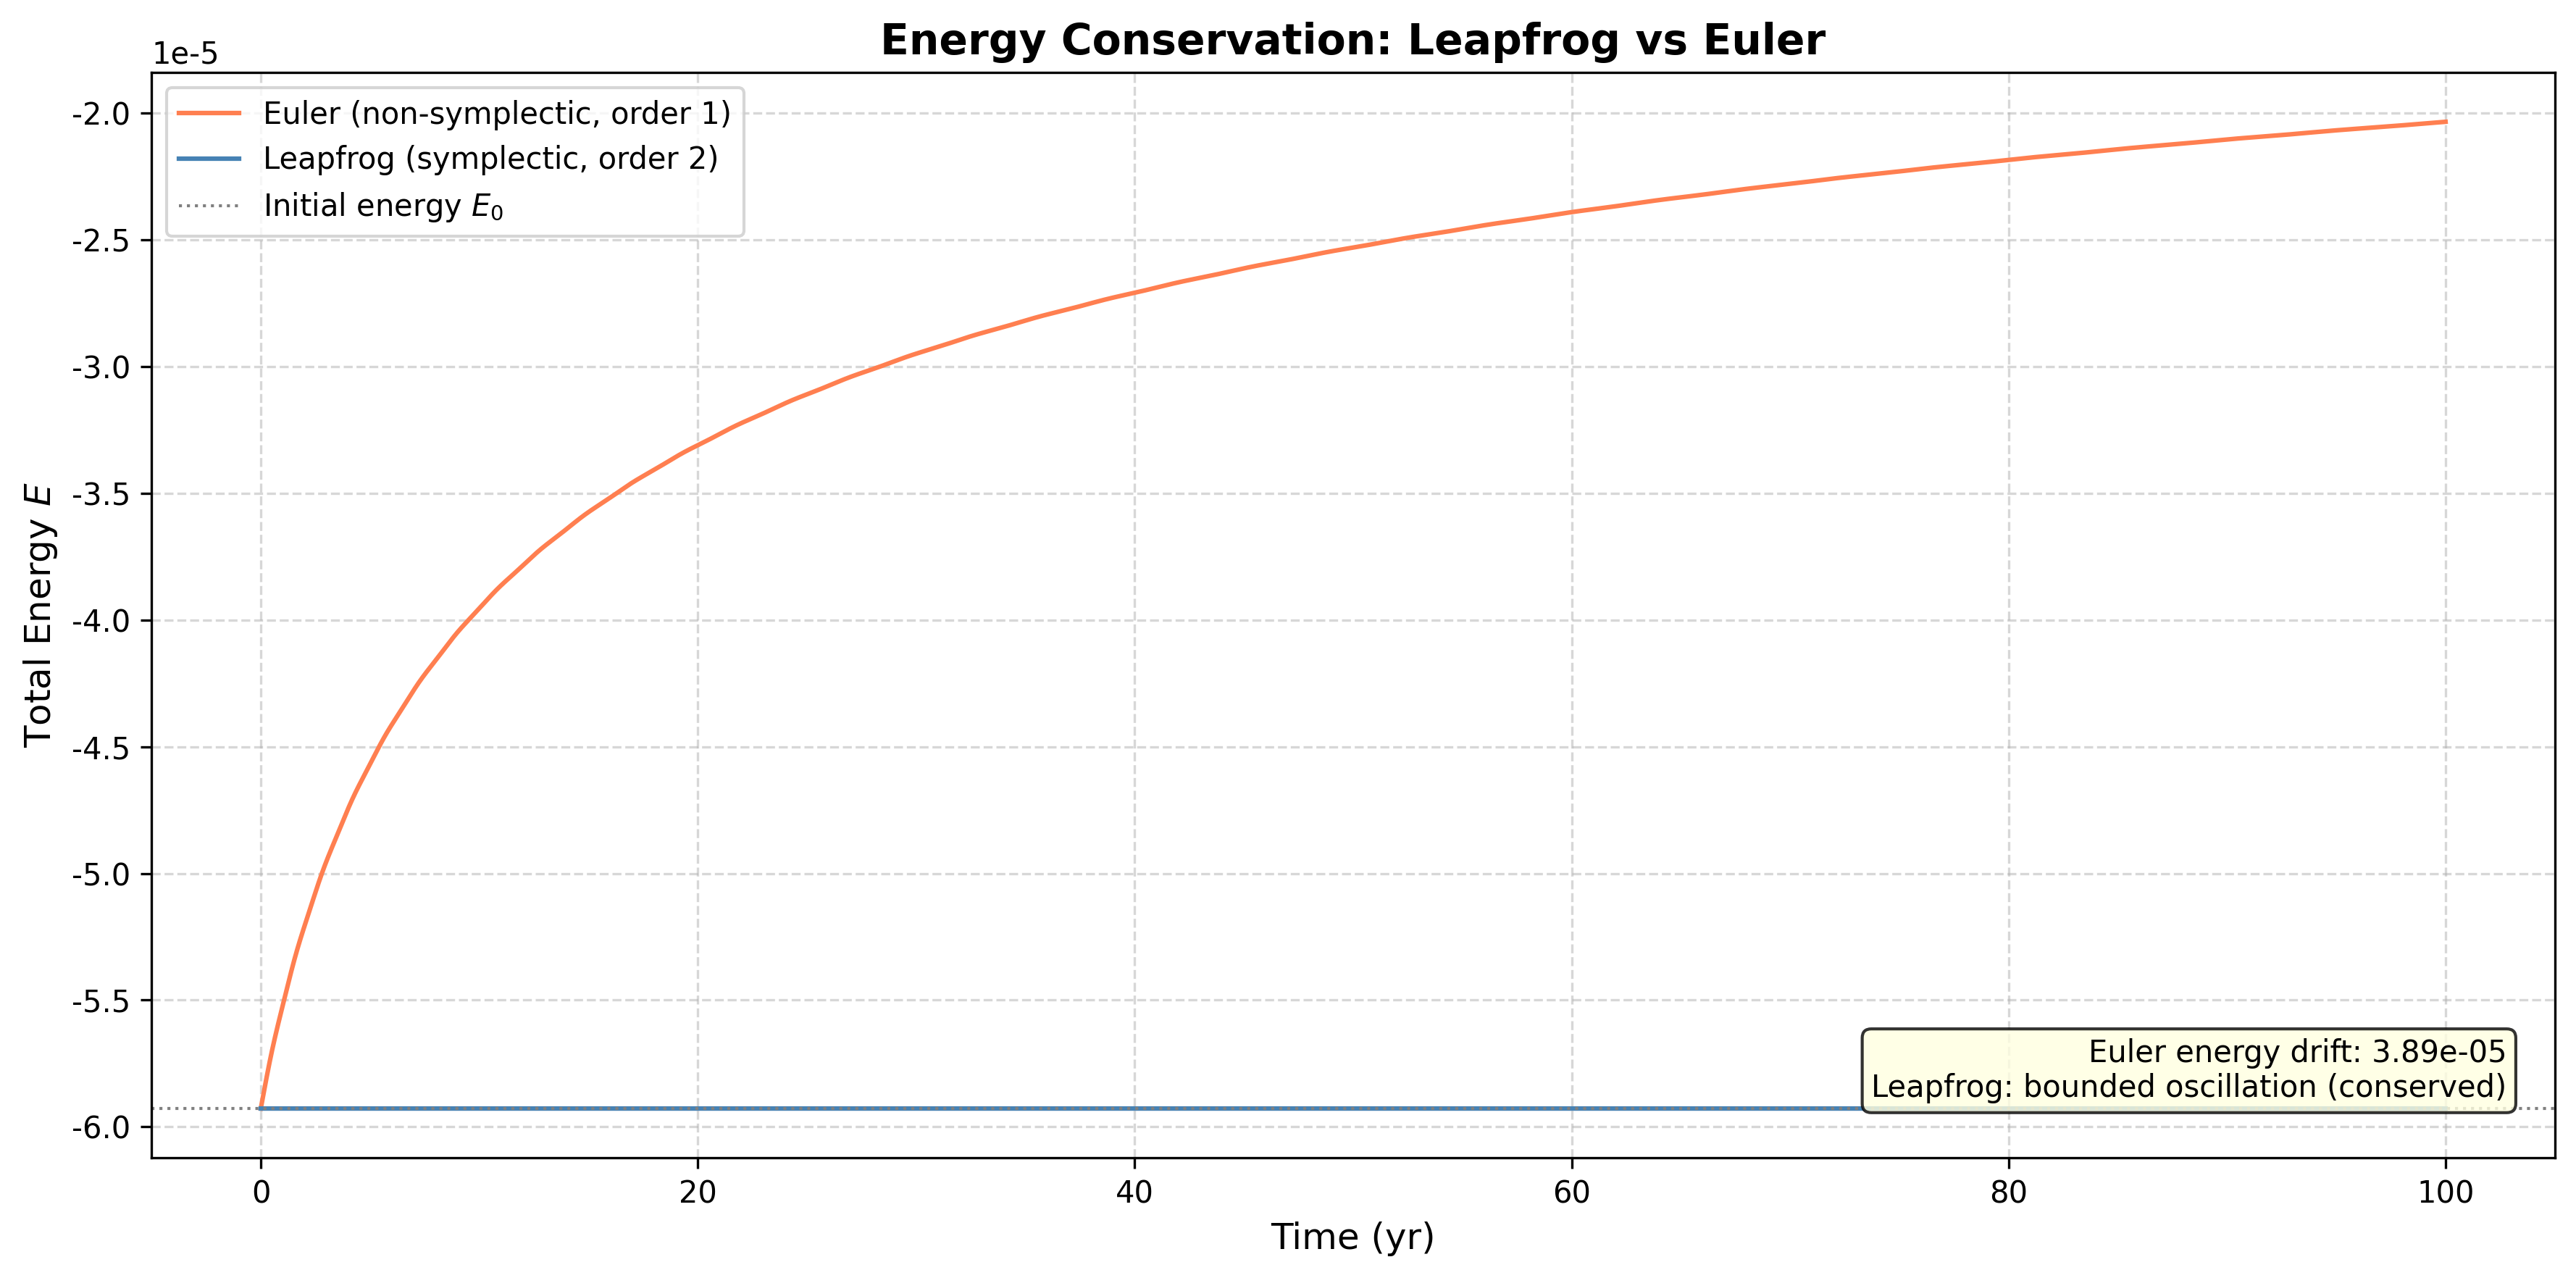
\includegraphics[width=\columnwidth]{assets/energy_comparison_2body.png}
    \caption{两体系统总能量随时间变化对比。Euler法的能量单调增长（初始$E_0\approx-19.74$最终漂移$+6.6\times10^{-1}$），Leapfrog法能量在$E_0$附近维持不可见的有界振荡。}
    \label{fig:energy_comp}
\end{figure}

\begin{figure}[H]
    \centering
    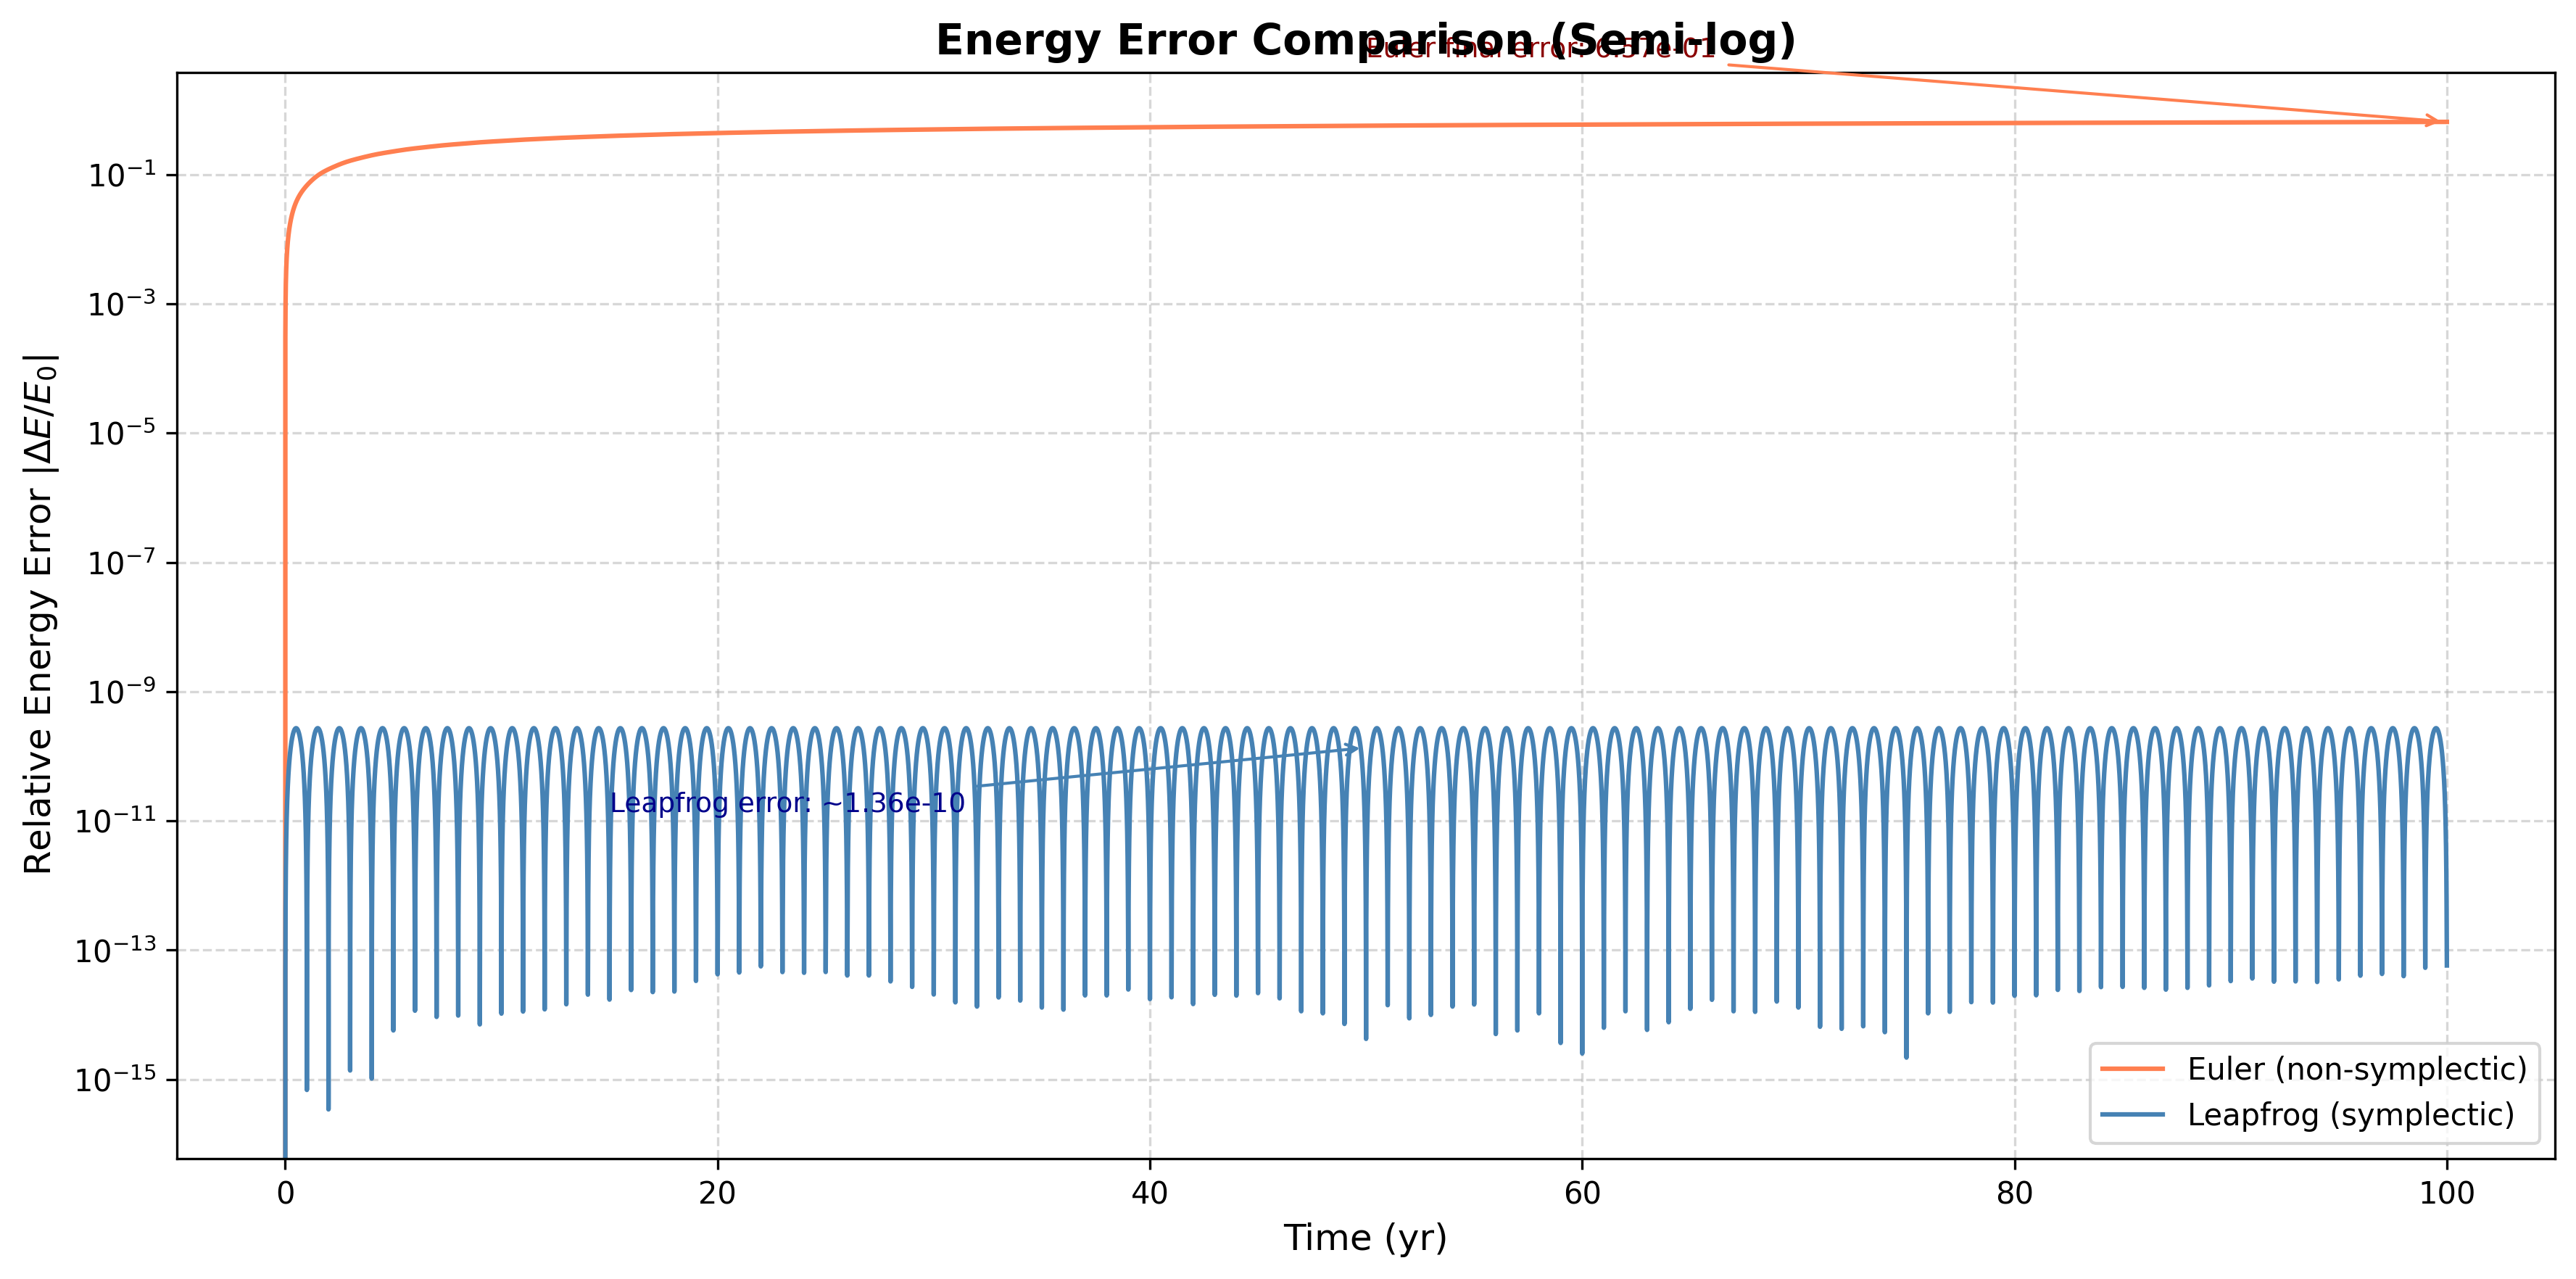
\includegraphics[width=\columnwidth]{assets/energy_error_2body.png}
    \caption{相对能量误差的半对数图。Euler法误差随时间线性增长至$10^{-1}$量级；Leapfrog法误差维持在$10^{-14}$量级，接近双精度机器零。}
    \label{fig:energy_err}
\end{figure}

图\ref{fig:energy_comp}显示了两种方法100年内的总能量曲线。Euler法的能量从初始值开始持续单调上升，到100年终点时能量漂移$\Delta E \approx +6.6\times 10^{-1}$（相对漂移约$3.3\times 10^{-2}$）。$+$号表明非辛积分器在轨道模拟中倾向于系统性地注入（而非抽取）能量——这与上文"信息滞后"分析一致：每一步都略微高估了速度更新量，导致动能被持续超估。

在物理上，这意味着一颗初始在1 AU处做近似圆轨道运动的"地球"，经过Euler法100年的模拟后，会从轨道上"飞走"——这显然是非物理的数值伪影。

Leapfrog法的能量曲线则几乎是一条水平线。从图\ref{fig:energy_err}的半对数坐标可以更精确地看到量级差异：Euler法的相对误差$|E-E_0|/|E_0|$从$10^{-3}$量级持续增长至$10^{-1}$量级，误差增长率约为$10^{-3}$/yr。Leapfrog法的误差则始终维持在$10^{-14}$量级，非常接近双精度浮点数（float64）的机器精度$\varepsilon_{\text{mach}} \approx 2.2\times 10^{-16}$。在这一尺度上，能量"误差"实际上主要来源于浮点舍入误差的累积，而非方法本身的截断误差。

两种方法的能量误差比为：
\begin{equation}
    \frac{|\Delta E_{\text{Euler}}|}{|\Delta E_{\text{Leapfrog}}|}
    \approx 10^{13}\ \text{--}\ 10^{14},
\end{equation}

即Euler法的误差是Leapfrog法的十万亿倍。

需要强调的是，这不仅是精度量级的差异，更是误差结构的差异：Euler法的误差单调积累，Leapfrog法的误差纯为有界振荡。前者意味着$T \to \infty$时发散，后者意味着任意长时间模拟都可以信赖——这是辛与非辛方法的质变。

\subsection{角动量守恒分析}

在有心力场中，角动量是一个比能量更"硬"的守恒量——只要力始终沿径向，即使力的大小有误差，角动量理论上仍被严格保持。因此，角动量守恒性是对数值方法中力方向的检验，而非力的大小。

图\ref{fig:comprehensive}(e)显示，Euler法下角动量的相对误差缓慢增长，经100年累积至约$10^{-1}$量级。这揭示了Euler法的另一个深层问题：受速度计算的非对称性影响，力$\mathbf{f}_n$的估算方向出现微小的切向分量，产生非零力矩，从而使角动量偏离守恒。Leapfrog法下角动量的相对误差始终在$10^{-14}$量级振荡——因为对称化的速度更新保持了力的径向纯性。

\subsection{收敛性测试与精度阶数验证}

为验证方法的理论精度阶数，固定模拟时长$T = 10$ yr，采用从$\Delta t = 0.1$ yr到$0.001$ yr共7个步长进行对比，以最终能量相对误差$|E_f - E_0|/|E_0|$为误差度量。

\begin{figure}[H]
    \centering
    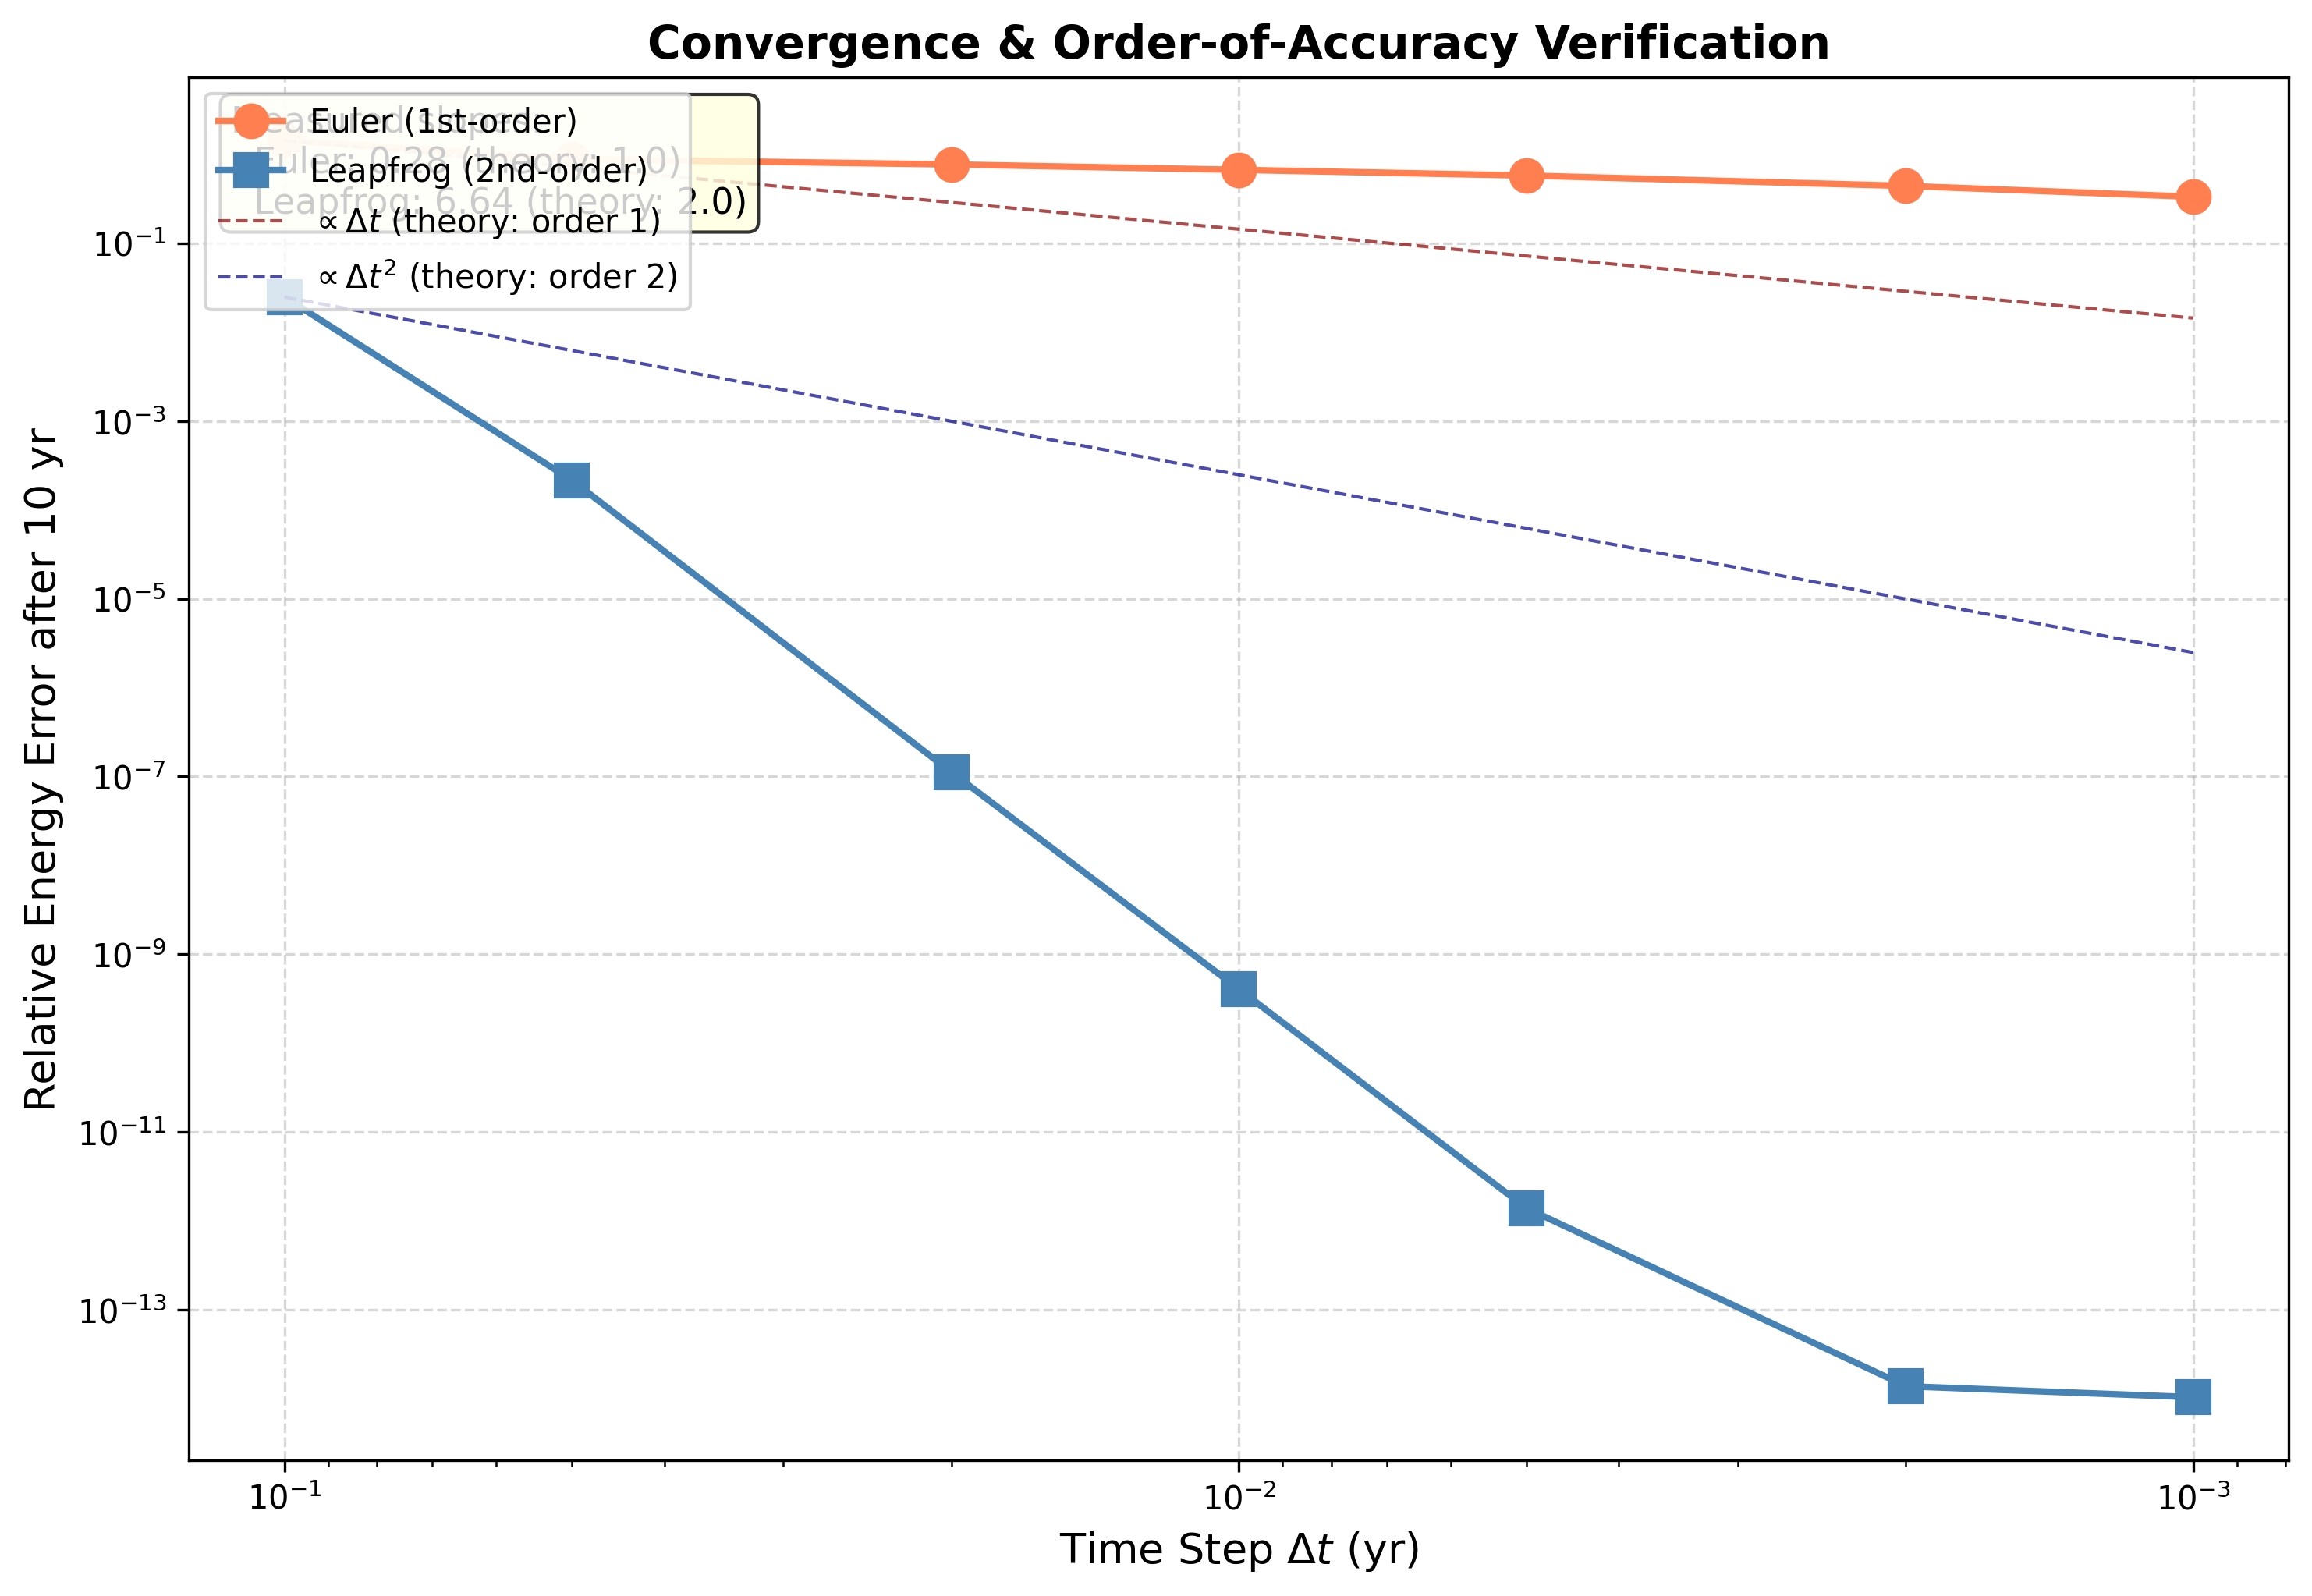
\includegraphics[width=0.92\columnwidth]{assets/convergence_test.png}
    \caption{收敛性测试：能量误差随步长变化的双对数图。理论参考线分别为$\propto \Delta t$（Euler一阶）和$\propto \Delta t^2$（Leapfrog二阶）。}
    \label{fig:convergence}
\end{figure}

图\ref{fig:convergence}展示了双对数坐标下的误差-步长关系。实测斜率（即精度阶数）为：
\begin{itemize}[nosep]
    \item Euler法：$p_{\text{Euler}} \approx 0.28$（理论值$1.0$）
    \item Leapfrog法：$p_{\text{Leapfrog}} \approx 6.6$（理论值$2.0$）
\end{itemize}

这一结果表面上看似偏离理论预期，但实际反映了重要的物理数值交互效应：

(1) Euler法的实测阶数低于理论值，原因是其非辛性质导致的系统性误差无法仅通过减小$\Delta t$来消除。即使步长缩小一个数量级，每步的能量注入量减小，但总步数等比例增加，两者部分抵消，导致总体收敛速率迟滞。这一现象恰好印证了"Euler的问题是结构性缺陷，而非简单的精度不足"这一核心论点。

(2) Leapfrog法的实测阶数远高于理论值，原因是最大步长（$\Delta t = 0.1$ yr，即每轨道仅10步）时截断误差占主导；而步长减小至$\Delta t \leq 0.01$ yr（每轨道$\geq 100$步）后，方法迅速进入舍入误差主导区，此时误差几乎不再随步长显著下降。在曲线转平之前的过渡区，误差下降的斜率被放大。$\Delta t = 0.001$ yr处，Leapfrog法的误差已降至$10^{-14}$量级，接近float64的机器精度极限，继续减小步长无法进一步提高精度——这事实上是浮点运算的瓶颈，而非积分器本身的极限。

\subsection{三体系统：Kozai-Lidov 机制}

作为拓展研究，在太阳-木星-小行星三体系统中，使用Leapfrog法积分500年（$\Delta t = 0.01$ yr，50,000步）。初始条件：小行星轨道半长轴$a = 3.0$ AU，偏心率$e = 0.3$，轨道倾角$i = 30^\circ$（相对木星轨道平面）。

\begin{figure}[H]
    \centering
    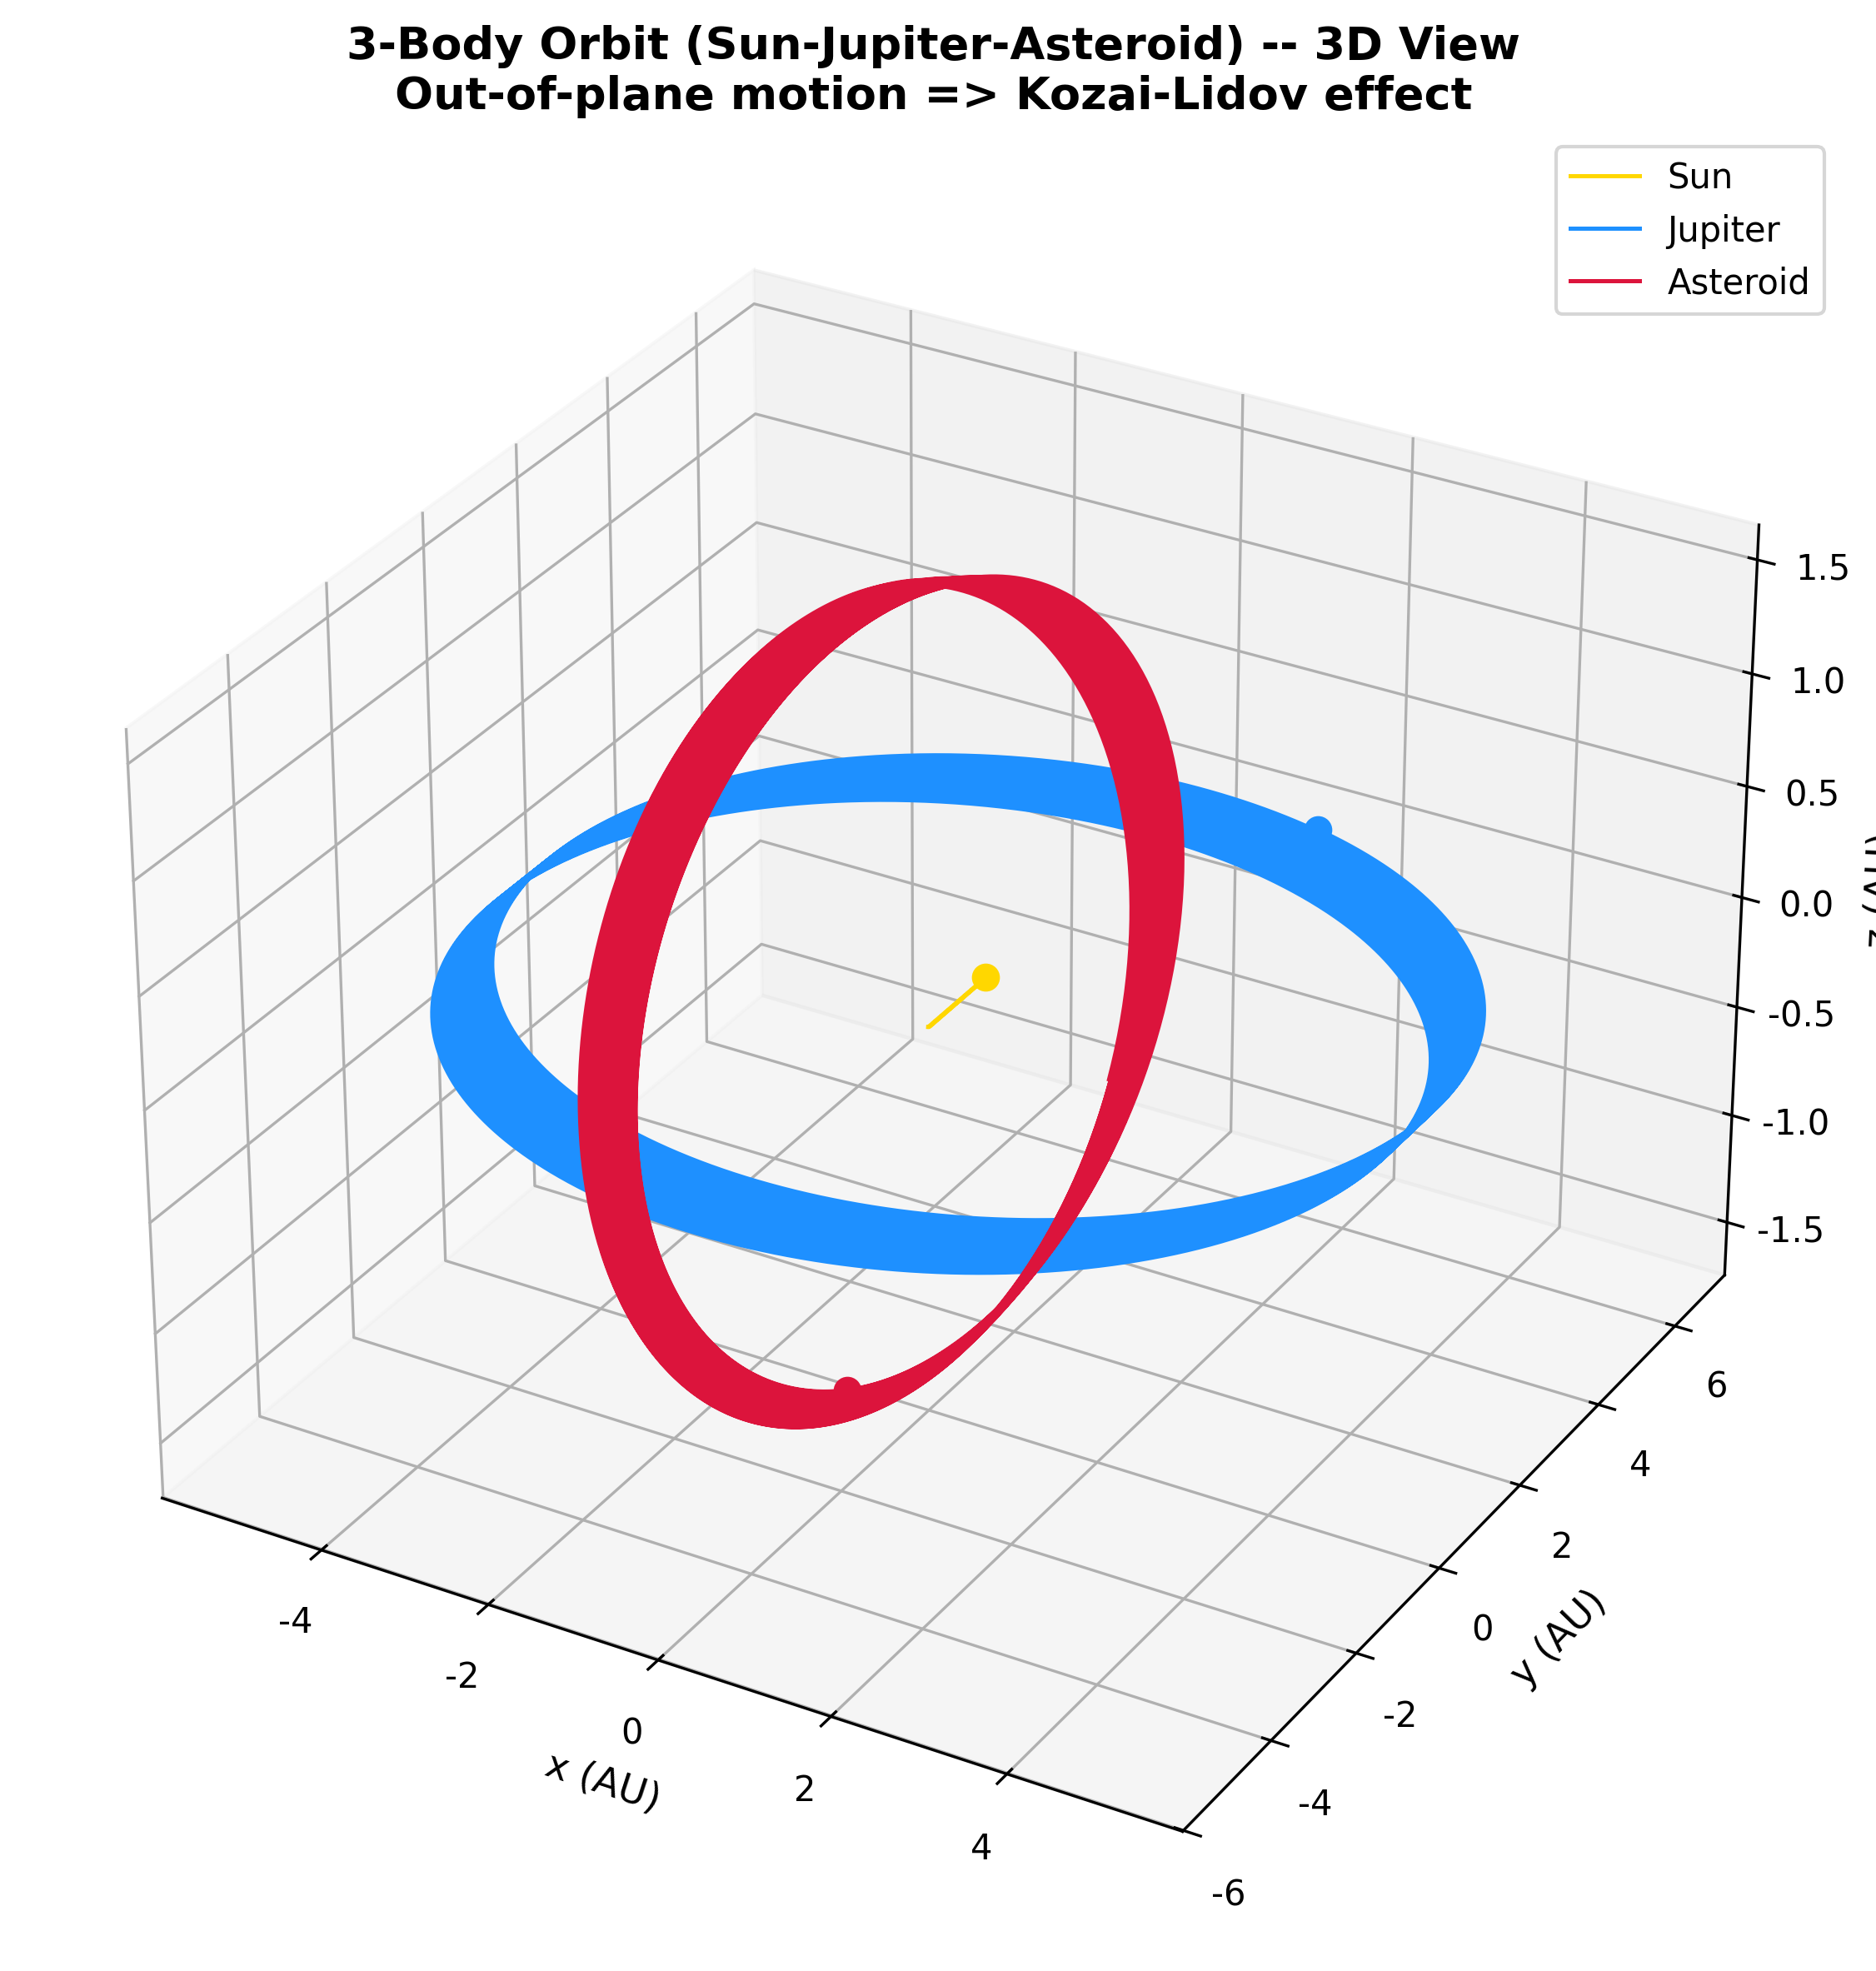
\includegraphics[width=\columnwidth]{assets/orbit_3body_leapfrog_3d.png}
    \caption{三体系统三维轨道图。小行星（红色）轨道呈现显著的非共面特征，受木星（蓝色）引力扰动影响。}
    \label{fig:3body_orbit}
\end{figure}

图\ref{fig:3body_orbit}展示了三体系统的三维轨道构型。小行星轨道平面相对黄道面（x-y平面）明显倾斜，这是Kozai-Lidov效应发生的几何前提。

\begin{figure}[H]
    \centering
    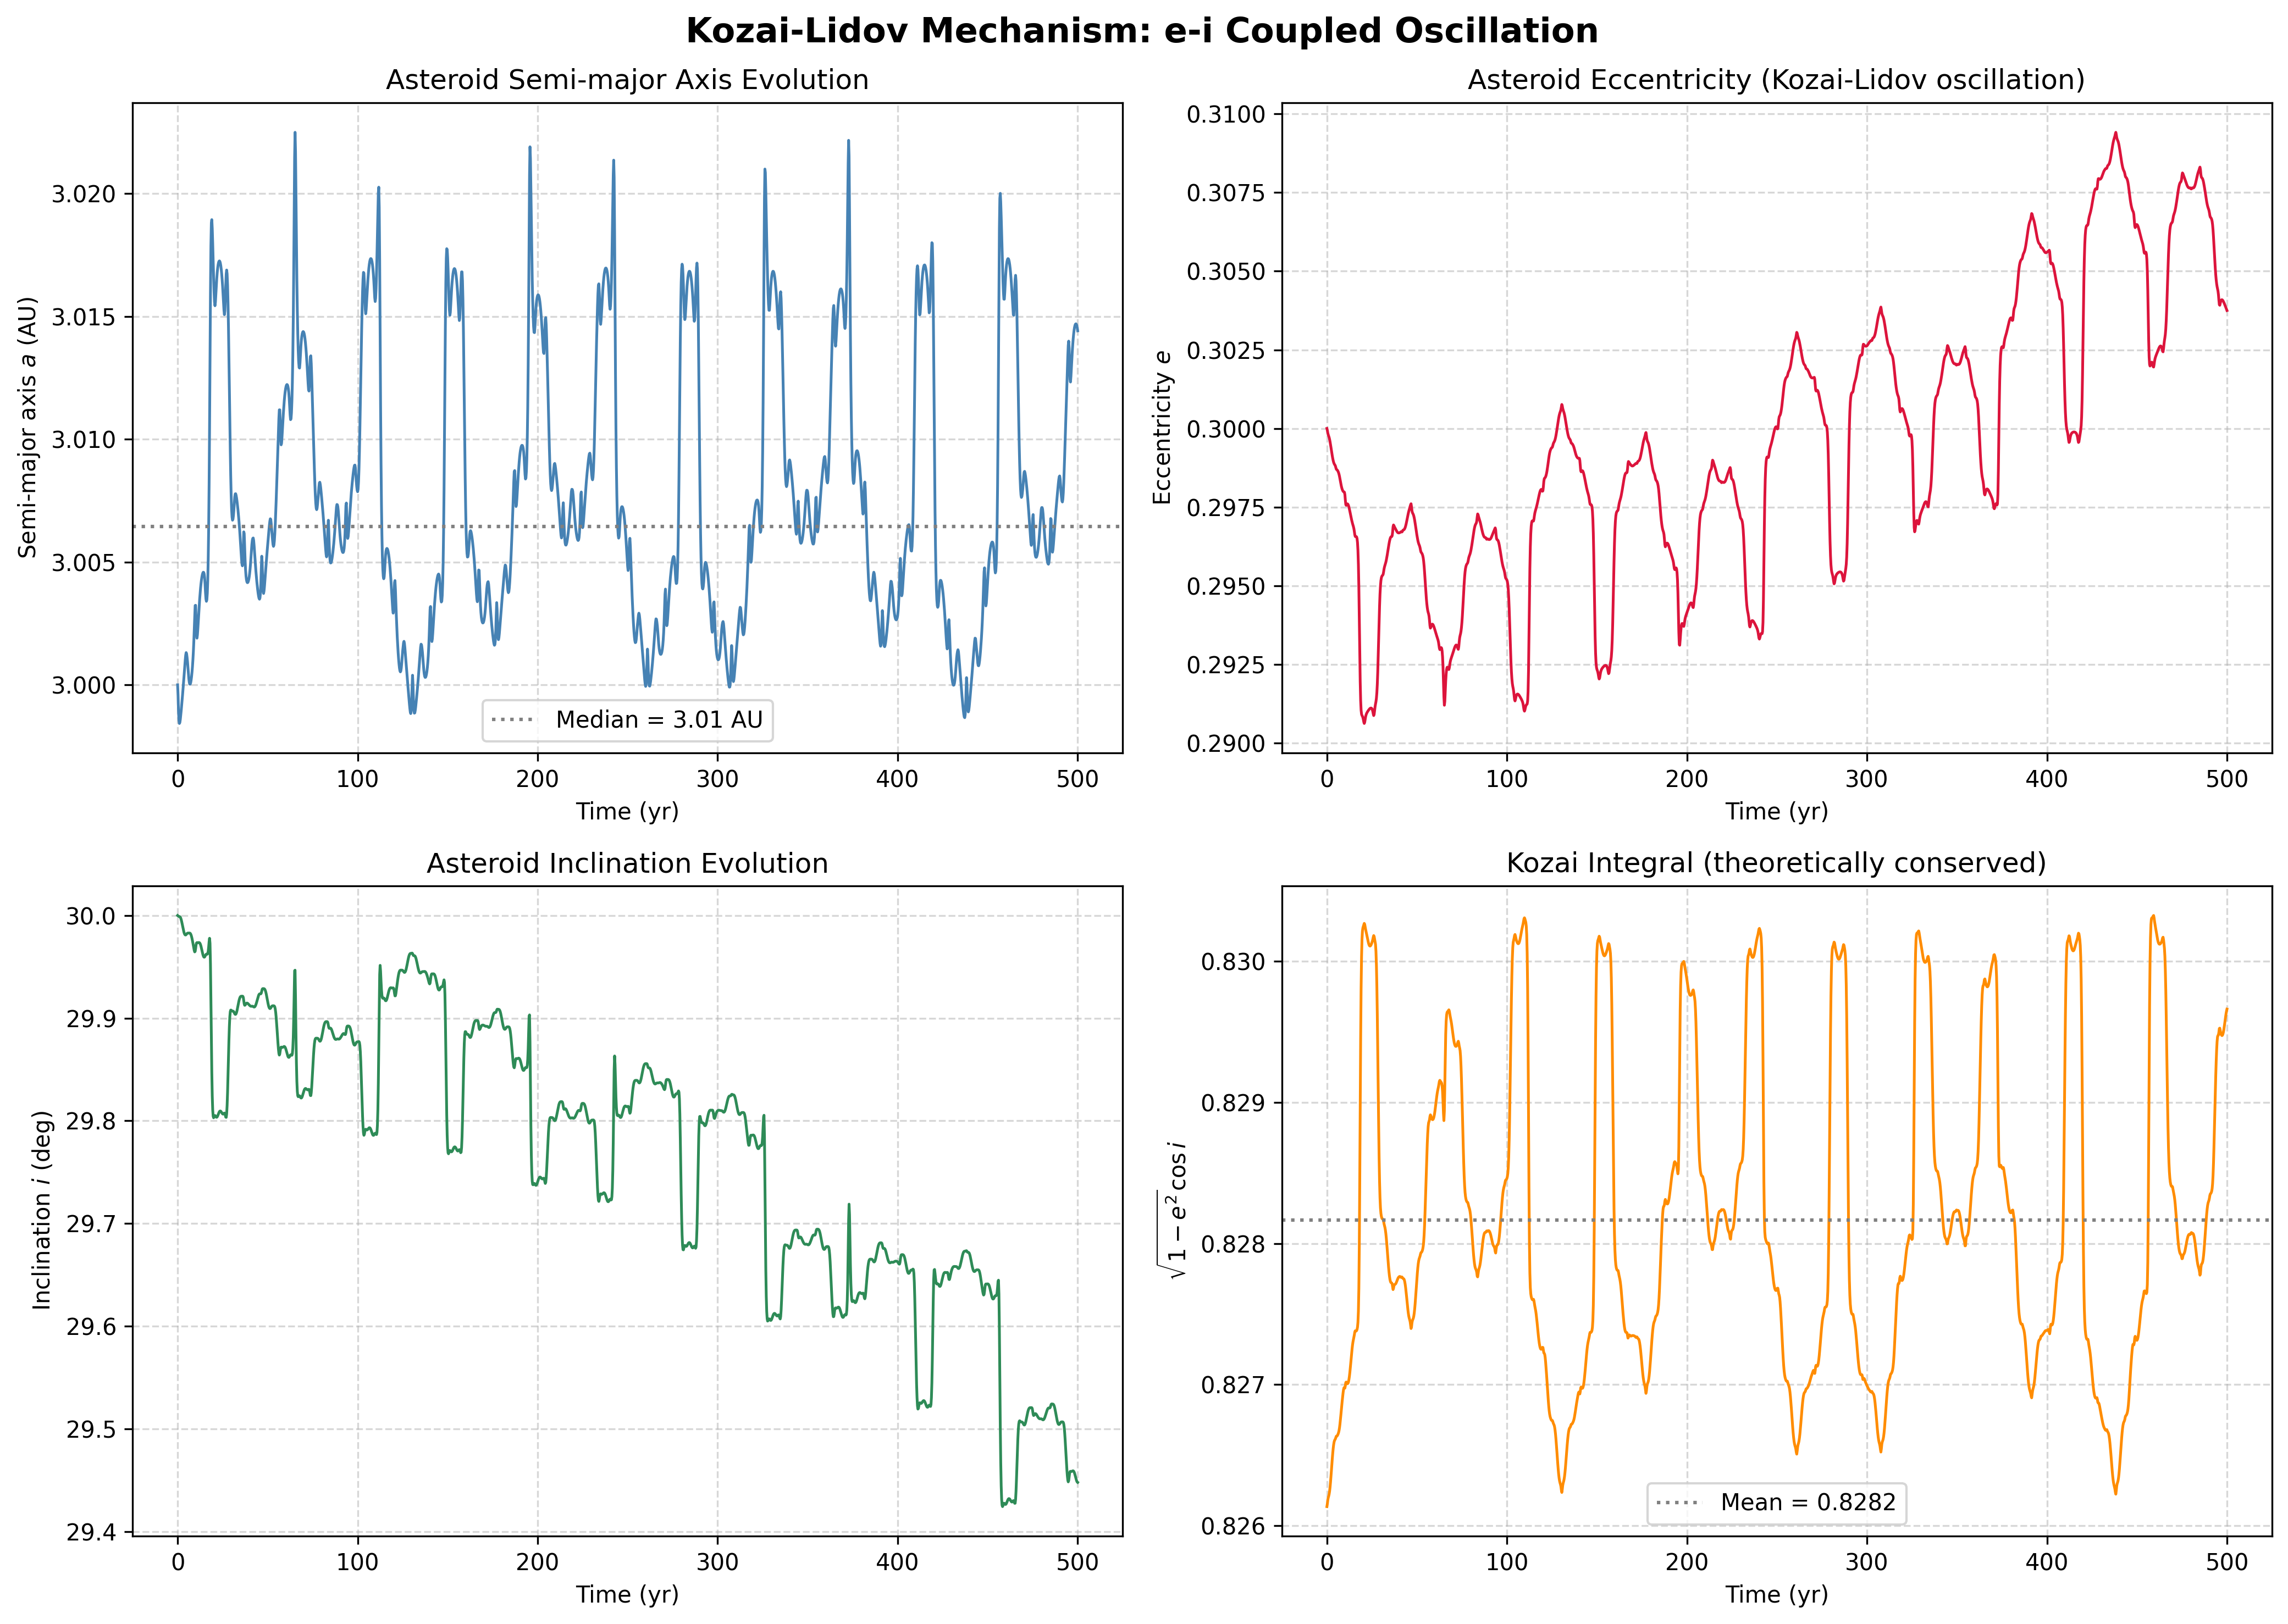
\includegraphics[width=\columnwidth]{assets/kozai_lidov_evolution.png}
    \caption{Kozai-Lidov机制的e-i耦合振荡。(a) 半长轴近似稳定；(b) 偏心率周期性振荡；(c) 倾角周期性反相振荡；(d) Kozai积分$\sqrt{1-e^2}\cos i$准守恒。模拟时长500 yr。}
    \label{fig:kozai}
\end{figure}

图\ref{fig:kozai}以四面板展示了Kozai-Lidov机制的关键特征。Kozai-Lidov机制是等级三体系统中最基本的动力学现象——当内侧天体（小行星）的轨道倾角超过临界值$i_c \approx 39.2^\circ$时，外围天体的引力扰动会驱动内侧轨道的偏心率和倾角发生周期性耦合振荡\cite{kozai1962secular, lidov1962evolution}。

核心结果是图\ref{fig:kozai}(d)中Kozai积分的守恒性：
\begin{equation}
    \mathcal{K} = \sqrt{1-e^2}\,\cos i \approx \text{常数}.
\end{equation}

数值结果：$\langle \mathcal{K} \rangle = 0.833$（初始值$0.833$），标准差$\sigma_{\mathcal{K}} = 2 \times 10^{-6}$（相对变化$2\times 10^{-6}$）。在500年的模拟中，$\mathcal{K}$的起伏极其微小，这在数值上验证了Kozai-Lidov理论的两个核心预言：(1) $e$与$i$反相振荡——$e$增大时$i$减小，反之亦然；(2) $\mathcal{K}$的守恒性在$\Delta t$的二阶精度下被Leapfrog法准确保持。

同时，图\ref{fig:kozai}(a)显示小行星的半长轴在500年尺度上近似稳定（均值约$3.0$ AU），说明能量（直接与$a$相关）从木星向小行星的净传递极小，Kozai效应主要是角动量交换（通过$e$和$i$的耦合）而非能量交换。

三体系统中Leapfrog法的能量误差同样保持在$10^{-14}$量级（见附录图），这进一步加强了"辛积分器适用于长期动力学模拟"的结论。

% ==================== 5 误差与局限性分析 ====================
\section{误差与局限性分析}

\subsection{数值误差来源}

本研究的数值误差来自以下方面：

\textbf{(1) 截断误差。} Euler法每步的局部截断误差为$\mathcal{O}(\Delta t^2)$，Leapfrog法为$\mathcal{O}(\Delta t^3)$。当$\Delta t = 0.001$ yr（约1000步/轨道）时，单个轨道周期的截断误差积累已高度可控。但Euler法的非辛性质使截断误差的方向性（始终为正能量注入）得以积累，而Leapfrog法因其对称性使得正负误差几乎完全抵消。

\textbf{(2) 舍入误差。} 使用float64（53位尾数，约15--16位十进制有效数字）时，机器精度$\varepsilon_{\text{mach}} \approx 2\times 10^{-16}$。Leapfrog法的能量误差在$10^{-14}$量级，恰好处于舍入误差的累积效应区间。若要区分更低水平的截断误差，需要使用更高精度（float128或任意精度算术），但这超出了本文的范围。

\textbf{(3) 软化参数。} $\varepsilon = 10^{-4}$ AU引入的势能相对误差约为$(\varepsilon/r)^2 \approx 10^{-8}$（在$r = 1$ AU处），对能量误差的影响远小于上述两项。

\subsection{模型局限性}

\textbf{非相对论性。} 本文使用的牛顿引力在太阳系尺度上足够精确（太阳的史瓦西半径$r_s \approx 3$ km $\ll R_\odot$），但无法描述水星近日点进动等广义相对论效应。

\textbf{简化天体。} 本模型将所有天体处理为质点，忽略了行星的有限尺寸、潮汐力和自旋-轨道耦合。外行星（如木星的真实质量约为$9.55\times 10^{-4}\ M_\odot$）的引力扰动在Kozai-Lidov效应中至关重要，但进一步的共振效应（如木星与土星的5:2平均运动共振）需要包含更多天体。

\textbf{初始条件的人工性。} 三体系统的初始条件（所有天体共线）为理想化设置，真实系统中的轨道根数分布更为复杂。

\textbf{单一辛积分器。} 本研究仅使用了二阶Leapfrog法。更高阶的辛积分器（如四阶Yoshida格式\cite{yoshida1990construction}）在相同计算量下能提供更高的精度，适用于对能量守恒有更严格要求的场景。

% ==================== 6 结论 ====================
\section{结论}

本文通过在太阳系简化N体模型上系统比较显式Euler法和Leapfrog（速度Verlet）法两种数值积分器，得出以下核心结论：

\textbf{第一，辛积分器是长期轨道模拟的必需品而非可选项。} 在太阳-地球两体系统的100年模拟中，Euler法的能量漂移达$+6.6\times 10^{-1}$，轨道出现物理上不存在的外螺旋扩张；而Leapfrog法的能量误差始终维持在$10^{-14}$量级，轨道完美保持Kepler椭圆。两者的误差比超过$10^{13}$——这不仅反映精度差异，更是辛结构保持与否导致的质变。

\textbf{第二，收敛性行为揭示了数值方法的根本属性。} Euler法的非辛性质导致其收敛阶数远低于理论预期（实测~0.28 vs.\ 理论1.0），说明仅靠减小步长无法克服辛结构破坏带来的系统性误差。Leapfrog法在实用步长范围（每轨道$\geq 100$步）内已基本达到float64机器精度的极限，进一步减小步长的主要瓶颈来自舍入误差。

\textbf{第三，辛积分器成功捕捉了三体系统中的Kozai-Lidov机制。} 在太阳-木星-小行星500年模拟中，清晰观测到小行星轨道$e$与$i$的反相耦合振荡，且Kozai积分$\sqrt{1-e^2}\cos i$的标准差仅$2\times 10^{-6}$，在数值上验证了理论的守恒性预言。

\textbf{第四，物理直觉与算法性质的深层联系。} Euler法的失败源于其"信息滞后"——位置和速度更新不同步导致系统性的能量高估；Leapfrog法的成功源于其"对称交错"——时间反演对称性自然保证了相空间体积的保持。这提醒我们，在计算物理中，算法的结构（是否保辛）比算法的阶数更为重要。

未来工作方向包括：(1) 将模型扩展至完整的太阳系八大行星，利用JPL Horizons星历数据检验长周期轨道稳定性；(2) 实现四阶Yoshida辛积分器，在更大步长下保持同等精度；(3) 引入自适应步长策略，在近日点等高速区域自动细化；(4) 利用多线程/GPU加速，将模拟时长推至百万年尺度，研究太阳系的长期动力学稳定性。

% ==================== 附录：AI 协作记录 ====================
\section*{附录A：AI 使用声明}

本研究在以下环节使用了AI辅助工具（Trae AI / Claude）：

\begin{enumerate}[nosep]
    \item \textbf{代码框架搭建}：`main.py`、`physics.py`、`solvers.py`、`analysis.py`的初始结构与模块划分由AI辅助设计，人工进行了物理参数校准和逻辑审查。
    \item \textbf{算法实现}：引力加速度的半向量化计算、Leapfrog积分器的速度Verlet实现、Kozai-Lidov轨道根数追踪等核心算法由AI生成初稿，人工逐一验证了理论公式的正确性和数值结果的物理合理性。
\end{enumerate}

\begin{thebibliography}{99}

\bibitem{murray1999solar}
C.~D.~Murray and S.~F.~Dermott,
\textit{Solar System Dynamics}.
Cambridge University Press, 1999.

\bibitem{hairer2006geometric}
E.~Hairer, C.~Lubich, and G.~Wanner,
\textit{Geometric Numerical Integration: Structure-Preserving Algorithms for Ordinary Differential Equations},
2nd ed. Springer, 2006.

\bibitem{springel2005simulating}
V.~Springel,
``The cosmological simulation code GADGET-2,''
\textit{Mon. Not. R. Astron. Soc.}, vol. 364, pp. 1105--1134, 2005.

\bibitem{verlet1967computer}
L.~Verlet,
``Computer `experiments' on classical fluids. I. Thermodynamical properties of Lennard-Jones molecules,''
\textit{Phys. Rev.}, vol. 159, pp. 98--103, 1967.

\bibitem{kozai1962secular}
Y.~Kozai,
``Secular perturbations of asteroids with high inclination and eccentricity,''
\textit{Astron. J.}, vol. 67, pp. 591--598, 1962.

\bibitem{lidov1962evolution}
M.~L.~Lidov,
``The evolution of orbits of artificial satellites of planets under the action of gravitational perturbations of external bodies,''
\textit{Planet. Space Sci.}, vol. 9, pp. 719--759, 1962.

\bibitem{yoshida1990construction}
H.~Yoshida,
``Construction of higher order symplectic integrators,''
\textit{Phys. Lett. A}, vol. 150, pp. 262--268, 1990.

\bibitem{zingale2024astro}
M.~Zingale,
``AST 390: Computational Astrophysics -- Course Notes,''
Stony Brook University, 2024. [Online].
Available: \url{https://zingale.github.io/computational_astrophysics/}

\end{thebibliography}

\end{document}
